\documentclass{beamer}
\usepackage[german,english]{babel}
\usepackage[utf8]{inputenc}

\usepackage{graphicx}
%\usepackage{svg}
%\usepackage{wrapfig}
%\usepackage{eurosym}
%\usepackage{tabularx}
%\usepackage{multirow}
%\usepackage{listings}
%\usepackage{color}
\usetheme{Darmstadt}
% Other valid themes
%   Antibes, Bergen, Berkeley, Berlin, Copenhagen
%   Darmstadt, Dresden, Frankfurt, Goettingen, Hannover
%   Ilmenau, JuanLesPins, Luebeck, Madrid, Malmoe
%   Marburg, Montpellier, PaloAlto, Pittsburgh, Rochester
%   Singapore, Szeged, Warsaw, boxes, default

\usecolortheme{default}
% Other valid color schemes
%    albatross, beaver, beetle, crane, dolphin
%    dove, fly, lily, orchid, rose, seagull
%    seahorse, whale and the one and only wolverine

\title[Project 1]{Project 2}
\subtitle{Least squares regression and nearest neighbor classifiers}
\author{Lukas Drexler, Leif Van Holland, Reza Jahangiri, Mark Springer, Maximilian Thiessen}
\institute[Universität Bonn]{Rheinische Friedrich-Wilhelms-Universität}
\date{\today}

\begin{document}
	
\begin{frame}%1
	\titlepage
\end{frame}

%no table of contents not enough content for that
%\begin{frame}%2
%\frametitle{Table of Contents}
%\tableofcontents%[pausesections]
%\end{frame}


\section{Task 2.1}

\begin{frame}
\frametitle{Least squares regression for missing value prediction}
Height and weight data:
\begin{align*}
	\mathbf{x} = [x_1,...,x_n]^T \text{ and } \mathbf{y} = [y_1,...,y_n]^T\\
\end{align*}
Fit polynomials:
\begin{align*}
	y(x) = \sum_{j=0}^{d}w_jx^j
\end{align*}
Use least squares method with Vandermonde matrix:
\begin{align*}
\begin{pmatrix}
1 & x_0 & x_0^2 & \cdots & x_0^n \\ 
1 & x_1 & x_1^2 & \cdots & x_1^n \\
\vdots & \vdots & \vdots & \ddots &\vdots \\
1 & x_n & x_n^2 & \cdots & x_n^n \\ 
\end{pmatrix}\\
\end{align*}
\end{frame}

%\begin{frame}
%\frametitle{Results for $d\in \{1,5,10\}$}
%\begin{figure}
%	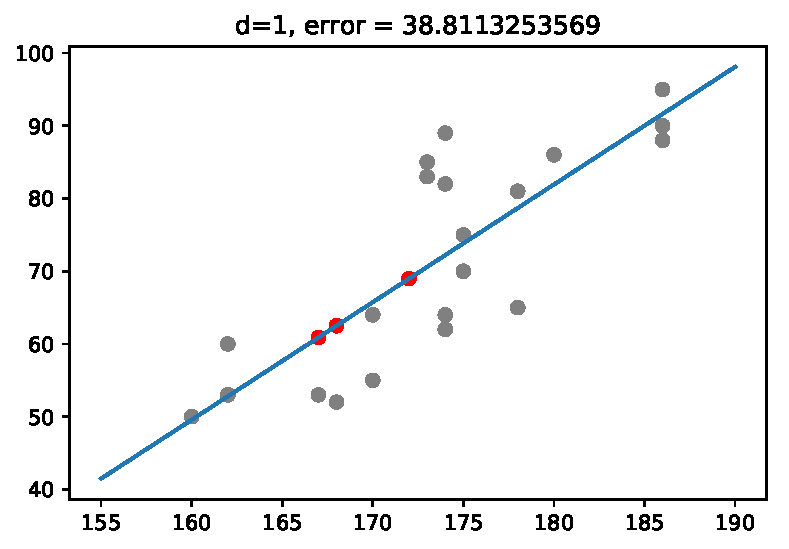
\includegraphics[height=0.5\textheight]{graphics/poly_1_coeffs}
%\end{figure}
%\end{frame}
\begin{frame}
\centering
\begin{tabular}{c}
	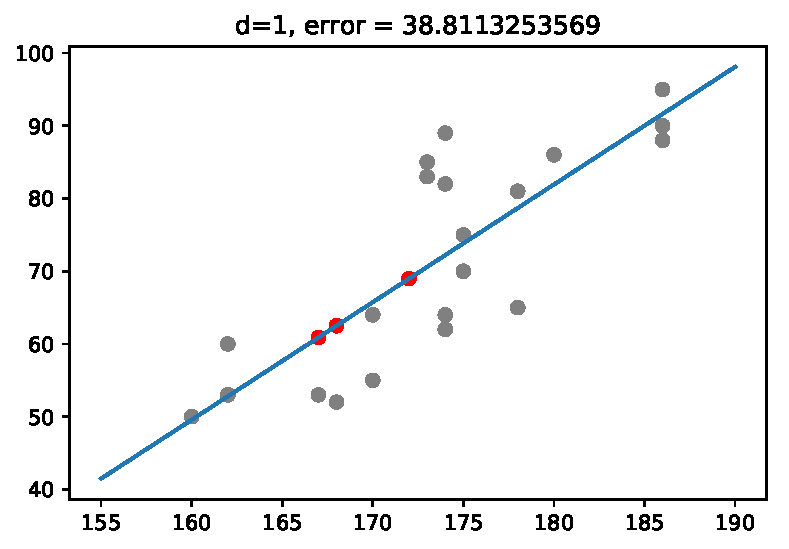
\includegraphics[width=6.5cm]{graphics/poly_1_coeffs}
\end{tabular}

\vspace{0.01em}
\begin{tabular}{cc}
	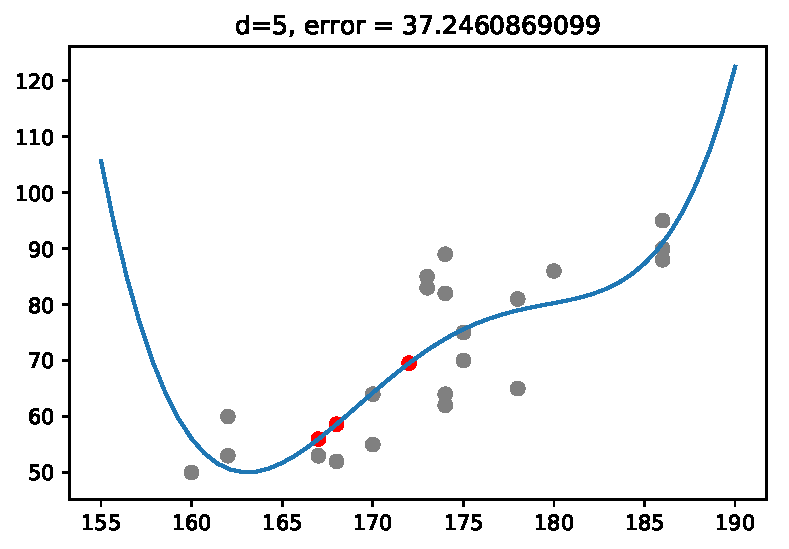
\includegraphics[width=5.5cm]{graphics/poly_5_coeffs}
	&
	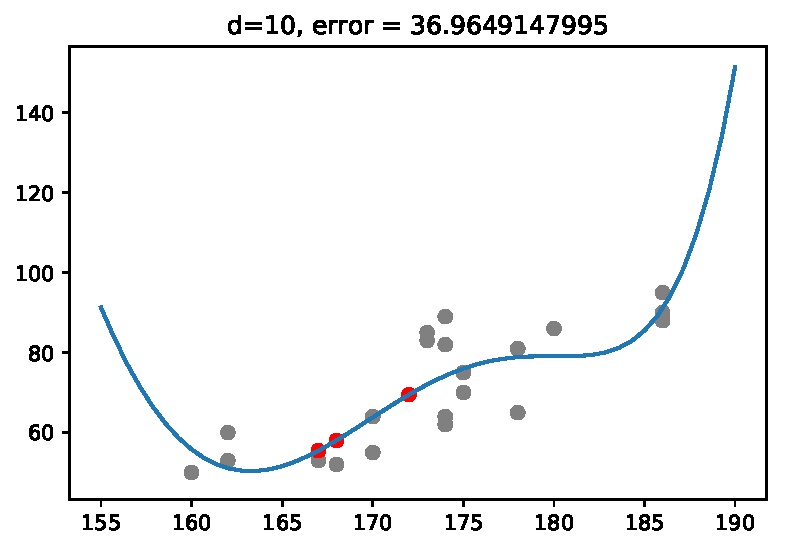
\includegraphics[width=5.5cm]{graphics/poly_10_coeffs}
\end{tabular}
\end{frame}

\section{Task 2.2}

\begin{frame}
	\frametitle{Conditional expectation for missing value prediction}
	Fit bi-variate Gaussian and use conditional Expectation for missing value prediction:
	\begin{align*}
		\mathbb{E}[w|h_0] &= \int w p(w|h_0) dw \\
						  &= \mu_w + \rho \frac{\sigma_w}{\sigma_h}(h_0-\mu_h)
	\end{align*}
\end{frame}

\begin{frame}
	\frametitle{Numeric Results}
	The red points have the predicted weight.
	\begin{figure}
		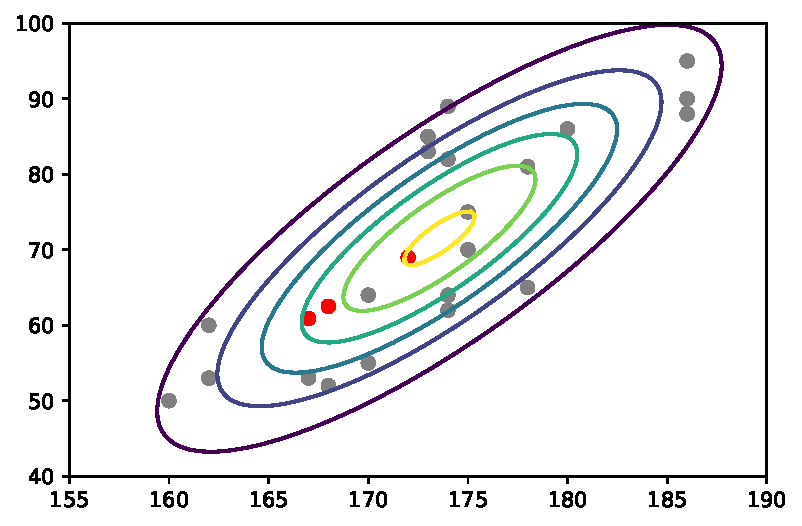
\includegraphics[width=0.9\linewidth]{graphics/contours}
	\end{figure}
\end{frame}

\section{Task 2.3}

\begin{frame}
	\frametitle{Bayesian regression for missing value prediction}
	Compare fifth degree polynomial
	\begin{align*}
		y(x) = \sum_{j=0}^{5}w_jx^j
	\end{align*}
	to a Bayesian regression assuming a Gaussian prior
	\begin{align*}
		p(\mathbf{w}) \sim \mathcal{N}(\mathbf{w}|\mu_0,\sigma^2_0\mathbf{I})
	\end{align*}
	with $\mu_0=\mathbf{0}$ and $\sigma^2_0=3$
	
\end{frame}

\begin{frame}
	\frametitle{Results}
	\begin{figure}
		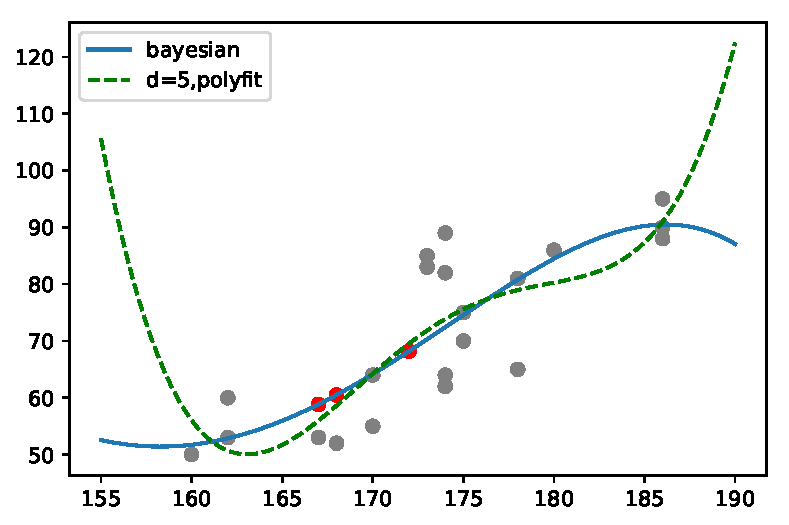
\includegraphics[height=0.85\textheight]{graphics/task3}
	\end{figure}
\end{frame}

\section{Task 2.4 (1)}
\begin{frame}
	\frametitle{Boolean functions and the Boolean Fourier transform}
\end{frame}
\section{Task 2.4 (2)}

\begin{frame}
	\frametitle{(Naive) $k$ nearest neighbor}
	Use the train data set as a prediction for the test data set \\\medskip
	Compute the $k$ nearest neighbors for each data point in the data set \\\medskip
	And use the majorant of those $k$ labels as a prediction \\\medskip
	Experiment on \texttt{data2.dat} with $k \in {1,3,5}$
\end{frame}

\begin{frame}
\frametitle{Results prediction}
	\begin{columns}[t]
	\column{.5\textwidth}
	\centering
	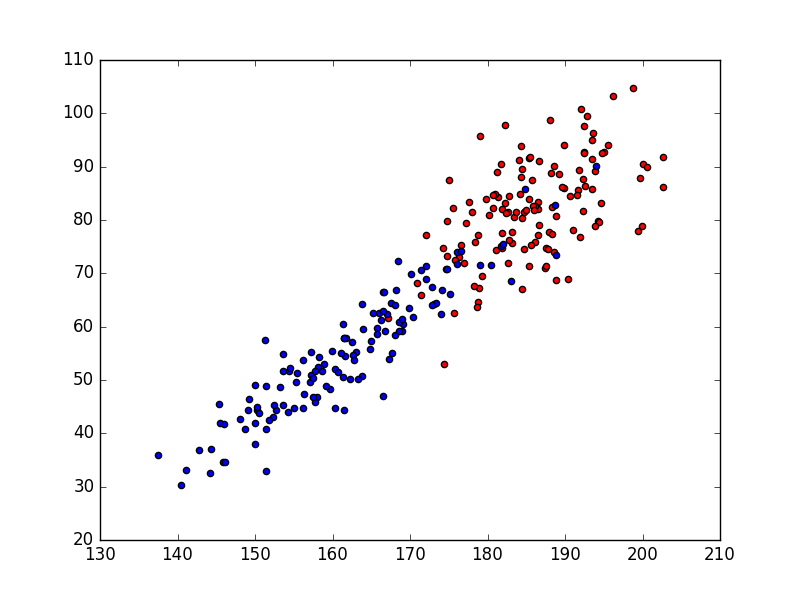
\includegraphics[width=5cm]{graphics/testWithCorrect}\\
	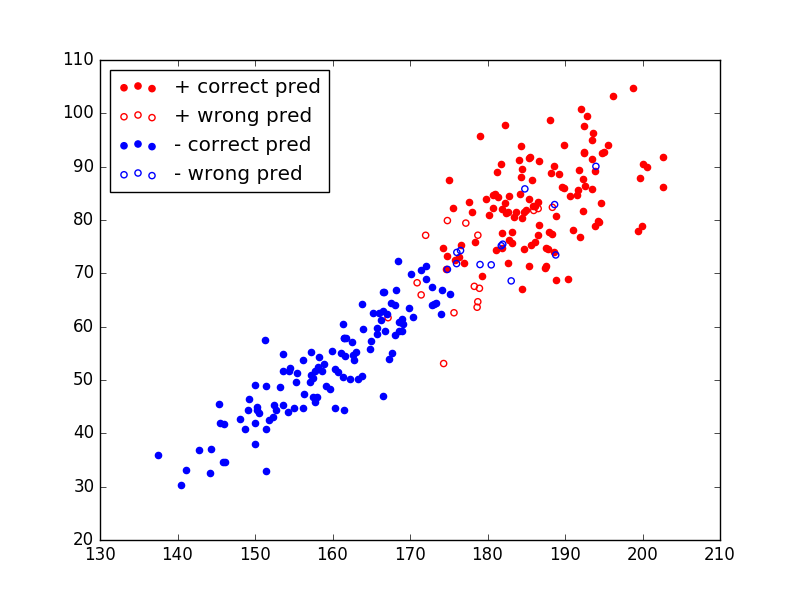
\includegraphics[width=5cm]{graphics/1NNPrediction}
	\column{.5\textwidth}
	\centering
	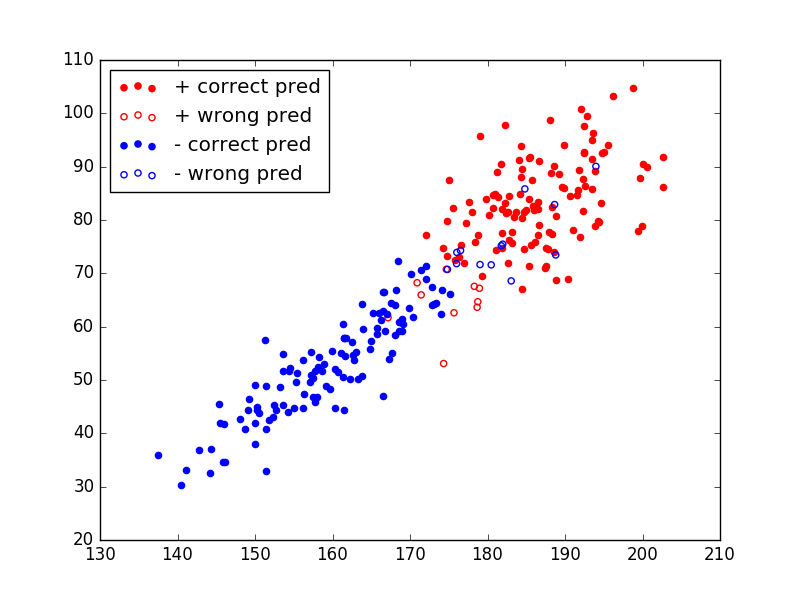
\includegraphics[width=5cm]{graphics/3NNPrediction}\\
	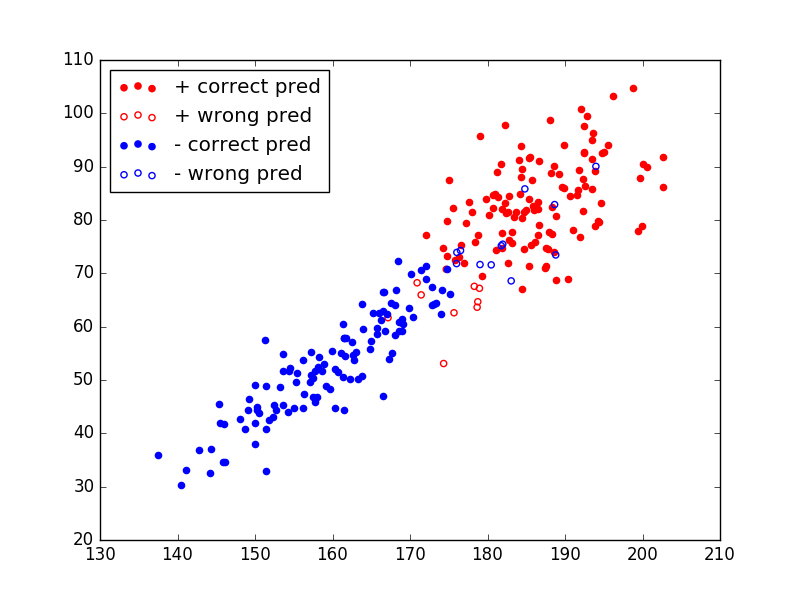
\includegraphics[width=5cm]{graphics/5NNPrediction}
\end{columns}
\end{frame}

\begin{frame}
\frametitle{Accuracy and running time}
Accuracies of $k$NN predictions:
	\begin{itemize}
		\item 0.77 for $k=1$
		\item 0.82 for $k=3$
		\item 0.83 for $k=5$
	\end{itemize}

Running times of our distance calculation vs \texttt{sklearn.metrics.pairwise}:
\begin{table}[]
	\centering
	\label{my-label}
	\begin{tabular}{l|l|l}
		k & our implementation &  \texttt{sklearn}\\ \hline
		1    & 0.02s & 0.003s \\ \hline
		3    & 0.02s & 0.003s \\ \hline
		5    & 0.02s & 0.003s \\ 
	\end{tabular}
\end{table}

\end{frame}

\section{Task 2.5}
\begin{frame}
	\frametitle{KDTrees}
	Plot four different KDTrees for combinations of  axis-cycling rules:
	\begin{itemize}
		\item[-] cycle through axes
		\item[-] select axis with highest variance
	\end{itemize}
	and the split point  rules w.r.t. the splitting axis:
	\begin{itemize}
		\item[-] select the median point
		\item[-] select the midpoint
	\end{itemize}
\end{frame}

\begin{frame}
	\begin{columns}[t]
		\column{.5\textwidth}
		\centering
		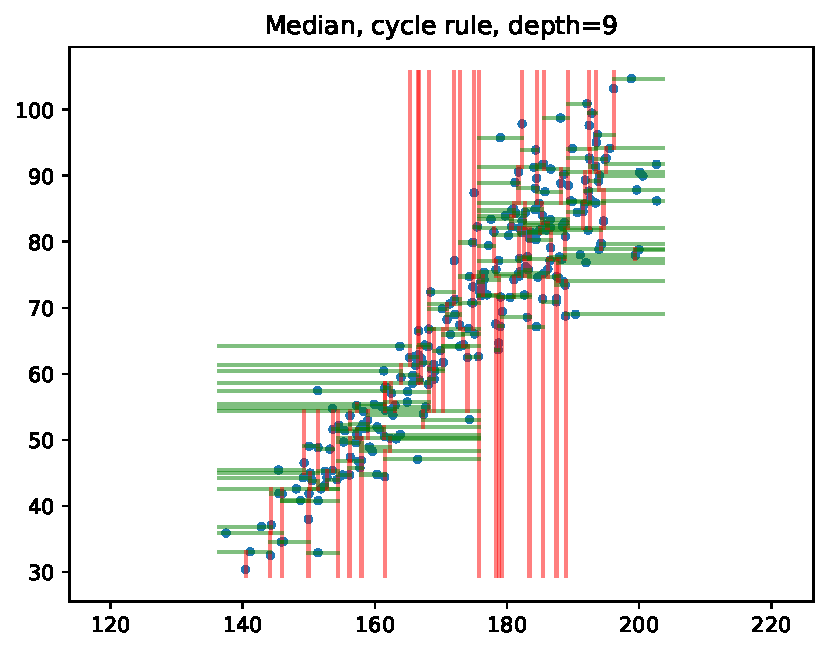
\includegraphics[width=5.5cm]{graphics/median_cycle}\\
		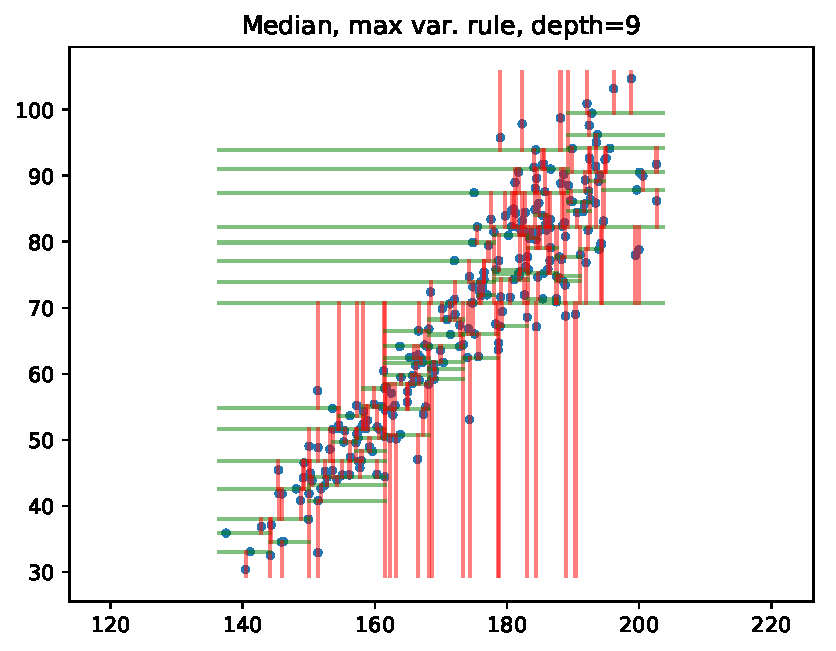
\includegraphics[width=5.5cm]{graphics/median_maxvar}
		\column{.5\textwidth}
		\centering
		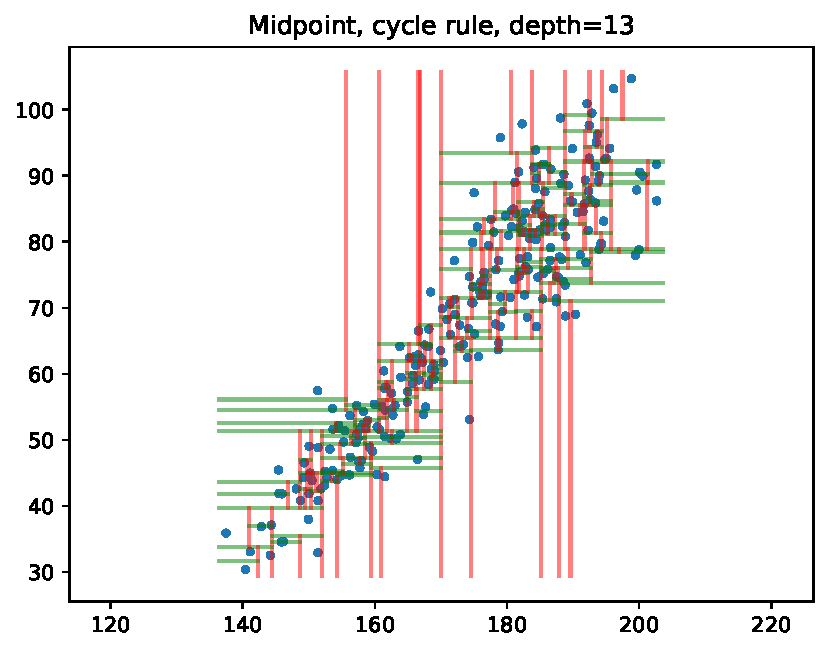
\includegraphics[width=5.5cm]{graphics/midpoint_cycle}\\
		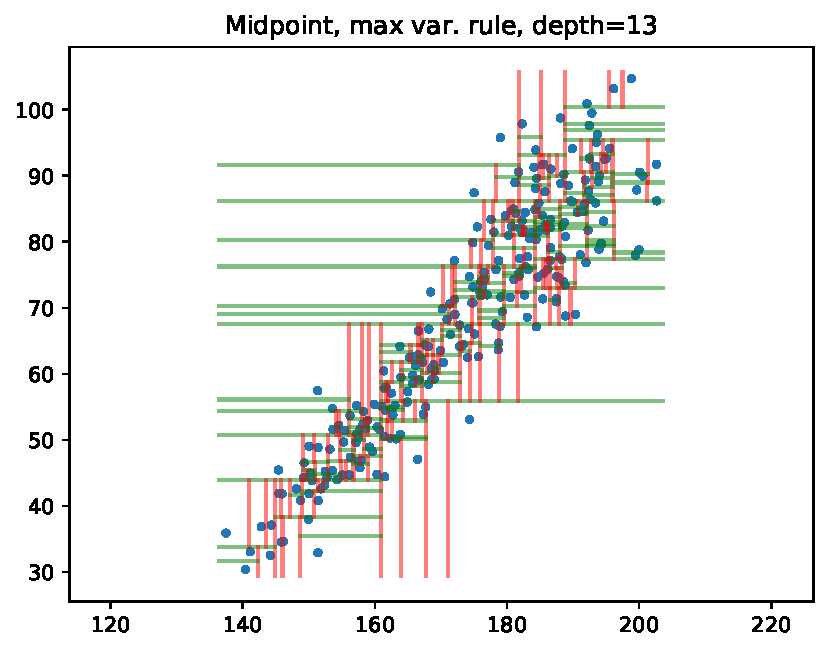
\includegraphics[width=5.5cm]{graphics/midpoint_maxvar}
	\end{columns}
\end{frame}

\begin{frame}
	\frametitle{Timings for 1-NN per combination}
	\begin{table}[]
		\centering
		\label{my-label}
		\begin{tabular}{l|l|l}
			& Median          & Midpoint        \\ \hline
			Cycle    & 0.0142476272583s & 0.0099373626709s \\ \hline
			Max. Var & 0.0136028242111s & 0.0105255293846s \\ 
		\end{tabular}
	\caption{Mean running time in seconds, 100 runs}
	\end{table}
\end{frame}



%\bibliography{Bibliography}
%\bibliographystyle{plain}

%\begin{thebibliography}{}
%\bibitem{1} 
%\bibitem{2} 
%\bibitem{3} 
%\end{thebibliography}


\end{document} 
